\section{Plot Types}


%%%%%%%%%%%%%%%%%%%%%%%%%%%%%%%%%%%%%%%%%%%%%%%%%%%
\subsection*{\href{\docurl\#pgfp./tikz/sharp:plot}{Line}}

\begin{wrapfigure}[5]{r}{2.2cm}
\vspace{-8mm}
\resizebox{2cm}{!}{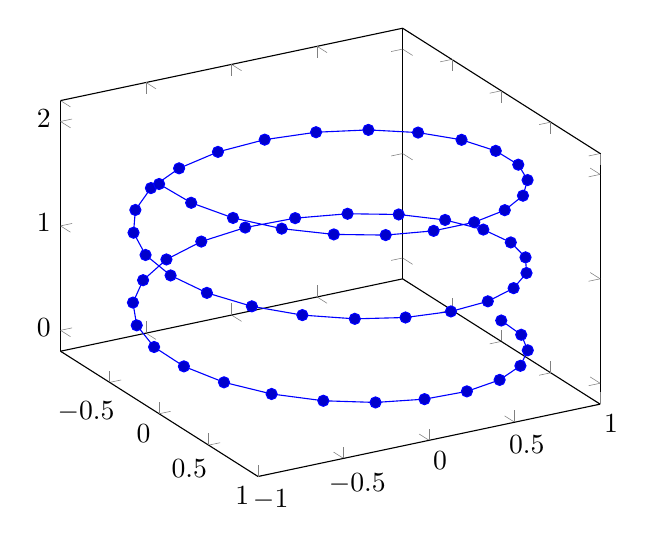
\begin{tikzpicture}
\begin{axis}[view={60}{30}]

\addplot3+ [domain=0:5*pi,samples=60,samples y=0,] ({sin(deg(x))},{cos(deg(x))},{2*x/(5*pi)});

\end{axis}
\end{tikzpicture}}
\end{wrapfigure}


\textit{Direct piecewise connections between samples are the default. Use }\opt{sharp plot}\textit{ to indicate explicitly, or change to }\href{\docurl\#pgfp./tikz/smooth}{\opt{smooth}}\textit{ for Bezier interconnections. Create \href{\docurl\#pgfp.back/addplot3}{3D line plots} by passing 3d tuples into }\texttt{\textbackslash addplot3}\textit{.}




%%%%%%%%%%%%%%%%%%%%%%%%%%%%%%%%%%%%%%%%%%%%%%%%%%%
\subsection*{\href{\docurl\#pgfp./pgfplots/hist}{Constant}}

\begin{wrapfigure}[5]{r}{2.2cm}
\vspace{-8mm}
\resizebox{2cm}{!}{\begin{tikzpicture} 
\begin{axis}
    \addplot+ [const plot,] coordinates {(0,0.1) (0.1,0.15) (0.4,0.56) (0.5,0.58) (0.6,0.65) (0.7,0.6) (0.8,0.58) (0.9,0.55) (1,0.52)};
\end{axis}
\end{tikzpicture}}
\end{wrapfigure}
\textit{Graphs with horizontal line connections. Options control placement of segments relative to coordinates, and whether vertical segments also shown.}

{\color{blue}
\begin{minipage}[t]{3.5cm}
const plot mark left\\
const plot mark right\\
const plot mark mid
\end{minipage}
\begin{minipage}[t]{2.8cm}
jump mark left\\
jump mark right\\
jump mark mid
\end{minipage}}



%%%%%%%%%%%%%%%%%%%%%%%%%%%%%%%%%%%%%%%%%%%%%%%%%%%
\subsection*{\href{\docurl\#pgfp./pgfplots/xbar}{Bar}}

\begin{wrapfigure}[5]{r}{2.2cm}
\vspace{-8mm}
\resizebox{2cm}{!}{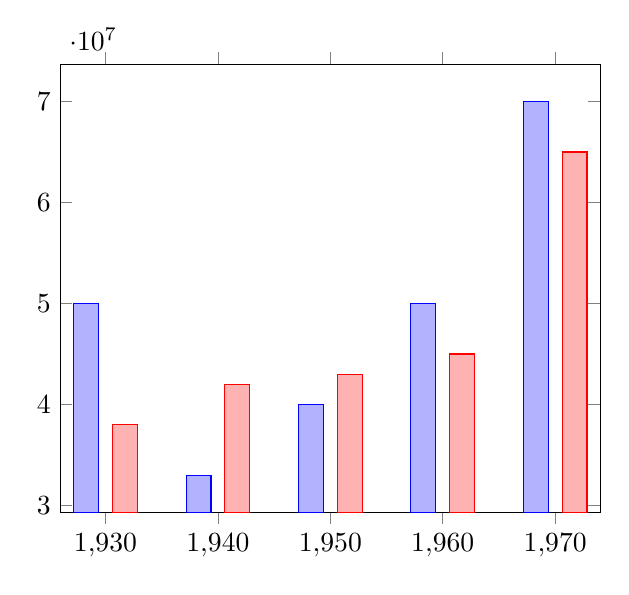
\begin{tikzpicture} \begin{axis}[
    %x tick label style={
    %    /pgf/number format/1000 sep=},
    %ylabel=Population, enlargelimits=0.15,
    %legend style={at={(0.5,-0.15)},
    %anchor=north,legend columns=-1}, 
    ybar=5pt,bar width=9pt,
    %nodes near coords,point meta=y *10^-7, % the displayed number
    ]
    \addplot coordinates {
        (1930,50e6) (1940,33e6)
        (1950,40e6) (1960,50e6) (1970,70e6)
    };
    \addplot coordinates {
        (1930,38e6) (1940,42e6)
        (1950,43e6) (1960,45e6) (1970,65e6)};
\end{axis}
\end{tikzpicture}
}
\end{wrapfigure}
\opt{[x|y]bar}\textit{, indicated at \underline{axis} level, affords bar charts in either x or y direction. Each }\texttt{\textbackslash addplot}\textit{ contributes an additional series. Options apply at axis level as well (except those marked with *):}

{\color{blue}
\begin{minipage}[t]{3.0cm}
xbar\\
ybar\\
bar shift auto\\
update limits
\end{minipage}
\begin{minipage}[t]{3.0cm}
bar width\\
enlarge [x|y] limits\\
pattern\\
bar cycle list
\end{minipage}}

\textit{Use }\opt{bar cycle list}\textit{ to install new styles for different series. A different graph altogether is }\opt{[x|y]bar interval}\textit{ which, together with }\opt{[x|y|z]ticklabel interval boundaries}\textit{ allows for bars of differing widths.}



%%%%%%%%%%%%%%%%%%%%%%%%%%%%%%%%%%%%%%%%%%%%%%%%%%%
\subsection*{\href{\docurl\#pgfp./pgfplots/hist}{Histogram}}

\begin{wrapfigure}[5]{r}{2.2cm}
\vspace{-8mm}
\resizebox{2cm}{!}{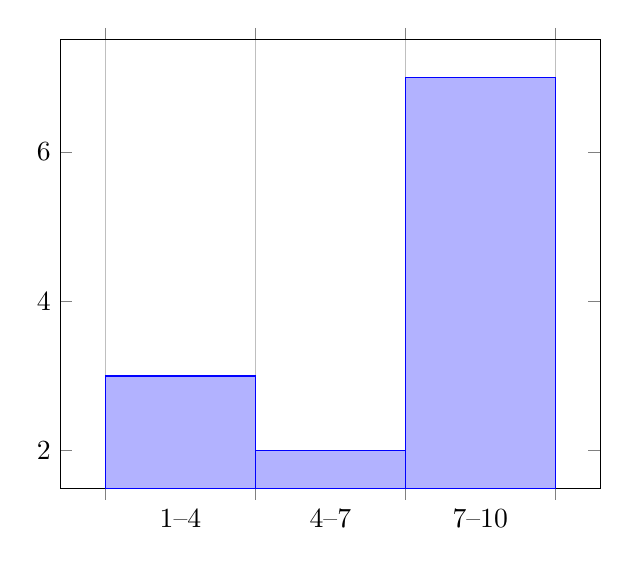
\begin{tikzpicture}
\begin{axis}[ybar interval,
    xticklabel=\pgfmathprintnumber\tick--\pgfmathprintnumber\nexttick
    ]

    \addplot+ [hist={bins=3}] table[row sep=\\,y index=0] {data\\1\\ 2\\ 1\\ 5\\ 4\\ 10\\7\\ 10\\ 9\\ 8\\ 9\\ 9\\};

\end{axis}
\end{tikzpicture}}
\end{wrapfigure}

\textit{Hist\textquotesingle s take }\texttt{addplot table}\textit{ or }\texttt{<expression>}\textit{ commands. Data must be single column.}\\
\code{\textbackslash addplot+ [hist=\{bins=3\}] }\\
\code{\phantom{xxx} table \dots }\\
\code{\textbackslash addplot+ [samples=200,hist] \{rnd\};}

{\color{blue}
\begin{minipage}[t]{3.0cm}
data\\
data min\\
data max\\
bins\\
symbolic coords\\
data coord trafo
\end{minipage}
\begin{minipage}[t]{3.0cm}
intervals\\
cumulative\\
density\\
handler\\
data filter\\
\end{minipage}}



%%%%%%%%%%%%%%%%%%%%%%%%%%%%%%%%%%%%%%%%%%%%%%%%%%%
\subsection*{\href{\docurl\#pgfp./pgfplots/box}{Box}}

\begin{wrapfigure}[5]{r}{2.2cm}
\vspace{-8mm}
\resizebox{2cm}{!}{\begin{tikzpicture}
\begin{axis}[boxplot/draw direction=y,]

\addplot+ [boxplot prepared={lower whisker=2.5,lower quartile=4,median=8.5,upper quartile=12,upper whisker=15},] coordinates{};

\addplot+ [  boxplot prepared={lower whisker=2.5,lower quartile=4,median=8.5,upper quartile=12,upper whisker=15},] coordinates{};

\addplot+ [  boxplot prepared={draw position=5,lower whisker=2.5,lower quartile=4,median=8.5,upper quartile=12,upper whisker=15},] coordinates{};

\end{axis}
\end{tikzpicture}}
\end{wrapfigure}

\textit{Can adjust orientation, box thickness, outlier distance, quartile thresholds, \say{whisker} styling, etc, with the following:}

{\color{blue}
\begin{minipage}[t]{3.0cm}
\end{minipage}
\begin{minipage}[t]{3.0cm}
\end{minipage}}



%%%%%%%%%%%%%%%%%%%%%%%%%%%%%%%%%%%%%%%%%%%%%%%%%%%
\subsection*{\href{\docurl\#pgfp./tikz/xcomb}{Comb}}


\begin{wrapfigure}[5]{r}{2.2cm}
\vspace{-8mm}
\resizebox{2cm}{!}{
\begin{tikzpicture}
\begin{axis}

    \addplot+ [xcomb,] coordinates{(4,0) (1,1) (2,2)(5,3) (6,4) (1,5)};

\end{axis}
\end{tikzpicture}}
\end{wrapfigure}

\textit{Similar to bar chart, but with lines rather than bars. As with bar, indicate with a set of coordinates:}\\
\code{\textbackslash addplot+[xcomb] coordinates \dots}\\


%%%%%%%%%%%%%%%%%%%%%%%%%%%%%%%%%%%%%%%%%%%%%%%%%%%
\subsection*{\href{\docurl\#pgfp./pgfplots/quiver}{Quiver}}


\begin{wrapfigure}[5]{r}{2.2cm}
\vspace{-8mm}
\resizebox{2cm}{!}{\begin{tikzpicture}
\begin{axis}[title=Quiver and plot table]
    \addplot[blue,
        quiver={u=\thisrow{u},v=\thisrow{v}},
        -stealth] 
	table 
	{
	x y u v
	0 0 1 0
	1 1 1 1
	2 4 1 4
	3 9 1 6
	4 16 1 8
	};
\end{axis}
\end{tikzpicture}}
\end{wrapfigure}

\textit{Requires a vector input $(u,v)$ that will calculate respective $(x,y)$ components of each \say{quiver. Works readily with parametrics (using }\texttt{variable=t}\textit{) \& tables of predefined $(x,y,u,v)$ vectors.} }\\

\begin{wrapfigure}[4]{l}{2.2cm}
\vspace{-6mm}
\resizebox{2cm}{!}{\begin{tikzpicture}
\begin{axis}
[title={$x \exp(-x^2-y^2)$ and its gradient},
domain=-2:2,
view={0}{90},
axis background/.style={fill=white},]

\addplot3 [contour gnuplot={number=9,labels=false},thick,] {exp(0-x^2-y^2)*x};
    
    \addplot3 [blue,-stealth,samples=15,quiver={u={exp(0-x^2-y^2)*(1-2*x^2)},v={exp(0-x^2-y^2)*(-2*x*y)},scale arrows=0.3,},] {exp(0-x^2-y^2)*x};
    
\end{axis}
\end{tikzpicture}
}
\end{wrapfigure}

\textit{Often used to visualize tangent \& gradient fields (using \href{\docurl\#pgfp./pgfplots/quiver/w}{3D quivers}). Set }\href{\docurl\#pgfp./pgfplots/quiver/w}{\opt{w}}\textit{ for 3rd dimension.}\\

{\color{blue}
\begin{minipage}[t]{1.0cm}
u\\
v\\
w\\
\end{minipage}
\begin{minipage}[t]{2.5cm}
colored\\
scale arrows\\
update limits\\
every arrow\\
\end{minipage}
\begin{minipage}[t]{2.2cm}
before arrow\\
after arrow\\
quiver legend
\end{minipage}}



%%%%%%%%%%%%%%%%%%%%%%%%%%%%%%%%%%%%%%%%%%%%%%%%%%%
\subsection*{\href{\docurl\#pgfp./pgfplots/stack:plots}{Stacked}}

\begin{wrapfigure}[5]{r}{2.2cm}
\vspace{-8mm}
\resizebox{2cm}{!}{
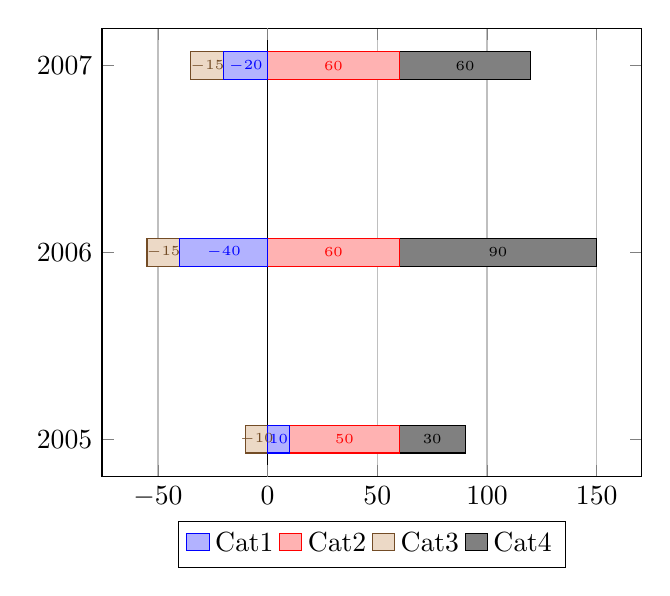
\begin{tikzpicture}
\pgfplotstableread{
    Year  Cat1  Cat2  Cat3  Cat4
    2005  10    50    -10   30
    2006  -40   60    -15   90
    2007  -20   60    -15   60
}\mytable

\begin{axis}[xbar stacked,% is default anyway:
stack negative=separate,%
/pgf/number format/1000 sep=,xmajorgrids,nodes near coords,nodes near coords style={font=\tiny},ytick distance=1,legend style={at={(0.5,-0.1)},anchor=north,legend columns=-1},extra x ticks={0},extra x tick style={grid style={black},xticklabel=\empty},]

    \addplot table[x index=1,y=Year] {\mytable};
    \addplot table[x index=2,y=Year] {\mytable};
    \addplot table[x index=3,y=Year] {\mytable};
    \addplot table[x index=4,y=Year] {\mytable};
    \legend{Cat1,Cat2,Cat3,Cat4}

\end{axis}
\end{tikzpicture}



\begin{comment}

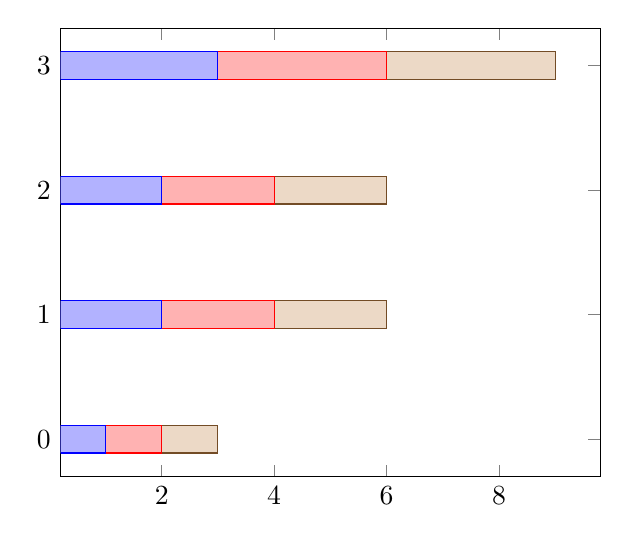
\begin{tikzpicture}
\begin{axis}[xbar stacked]

    \addplot coordinates{(1,0) (2,1) (2,2) (3,3)};
    \addplot coordinates{(1,0) (2,1) (2,2) (3,3)};
    \addplot coordinates{(1,0) (2,1) (2,2) (3,3)};
    
\end{axis}
\end{tikzpicture}

\end{comment}}
\end{wrapfigure}

\textit{Initiate basic stacking with }\href{\docurl\#pgfp./pgfplots/stack:plot}{\opt{stack plots}}\texttt{=y|x}\textit{, or stacked bars with, eg, }\href{\docurl\#pgfg./pgfplots/ybar:stacked}{\opt{ybar stacked}}\textit{. Given coordinates for each }\texttt{\textbackslash addplot}\textit{ line up positionally to comprise each of the plot\textquotesingle s \say{series\textquotesingle.} Can also stack in negative direction.}

{\color{blue}
\begin{minipage}[t]{2.5cm}
ybar stacked\\
xbar stacked\\
stack dir\\
stack negative
\end{minipage}
\begin{minipage}[t]{3.5cm}
reverse stacked plots\\
stacked ignores zero\\
xbar interval stacked\\
ybar interval stacked\\
bar shift auto
\end{minipage}}



%%%%%%%%%%%%%%%%%%%%%%%%%%%%%%%%%%%%%%%%%%%%%%%%%%%
\subsection*{\href{\docurl\#pgfp./pgfplots/z:buffer}{Mesh}}

\begin{wrapfigure}[5]{r}{2.2cm}
\vspace{-8mm}
\resizebox{2cm}{!}{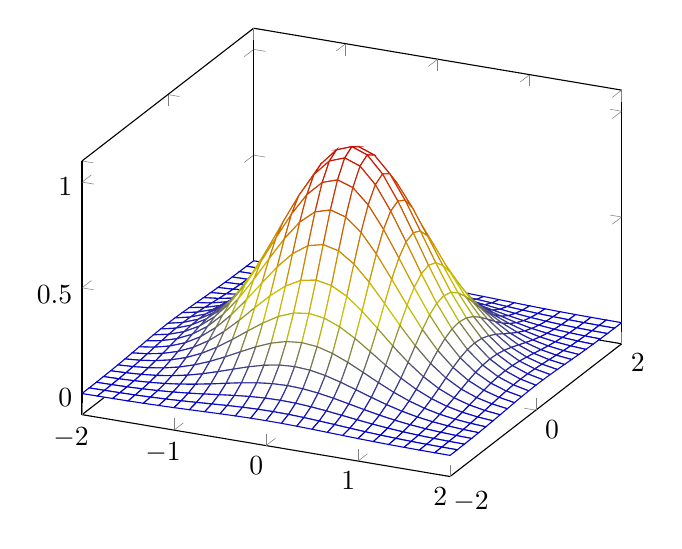
\begin{tikzpicture}
\begin{axis}
    []
    
    \addplot3 [surf,fill=white,domain=-2:2]
        {exp(-x^2-y^2)};
        
\end{axis}
\end{tikzpicture}}
\end{wrapfigure}

\textit{Available as 2D or, as is more customary, 3D. Invoke with }\href{pgfp\#./pgfplots/mesh}{\opt{mesh}}\textit{. Default mapping from $y$ to colormap. Change this using }\href{\docurl\#pgfp./pgfp/pgfplots/point:meta}{\opt{point meta}}\textit{.}




%%%%%%%%%%%%%%%%%%%%%%%%%%%%%%%%%%%%%%%%%%%%%%%%%%%
\subsection*{\href{\docurl\#pgfp./pgfplots/area:style}{Area}}



\begin{wrapfigure}[5]{r}{2.2cm}
\vspace{-8mm}
\resizebox{2cm}{!}{
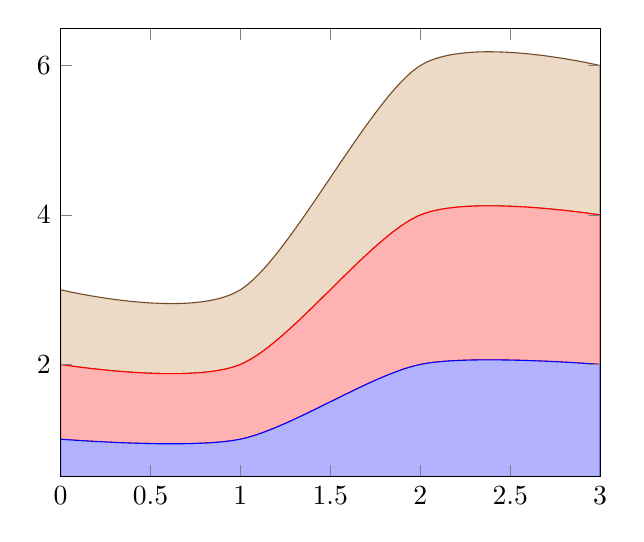
\begin{tikzpicture}
\begin{axis}[smooth,stack plots=y,area style,enlarge x limits=false,]

    \addplot coordinates{(0,1) (1,1) (2,2) (3,2)}\closedcycle;
    \addplot coordinates{(0,1) (1,1) (2,2) (3,2)}\closedcycle;
    \addplot coordinates{(0,1) (1,1) (2,2) (3,2)}\closedcycle;
    
\end{axis}
\end{tikzpicture}}
\end{wrapfigure}


\textit{For simple areas use stacking in addition to }\href{\docurl\#.pgfp/pgfplots/area:style}{\opt{area style}}\textit{. Can also use }\texttt{\href{\docurl\#pgfp.fill:between}{\textbackslash addplot fill between}}\textit{ in other plot types to achieve a fill affect, or use }\texttt{\href{\docurl\#pgfp.back/closedcycle}{\textbackslash closedcycle}}\textit{ at end of }\texttt{\textbackslash addplot}\textit{ to close a drawn path. Further restrict areas  by setting }\href{\docurl\#pgfp.soft:clip}{\opt{soft clip}}\textit{ key to a previously-defined \say{clip.}}





%%%%%%%%%%%%%%%%%%%%%%%%%%%%%%%%%%%%%%%%%%%%%%%%%%%
\subsection*{\href{\docurl\#pgfp./pgfplots/scatter}{Scatter}}


\begin{wrapfigure}[5]{r}{2.2cm}
\vspace{-8mm}
\resizebox{2cm}{!}{
\begin{tikzpicture}
\begin{axis}
[scatter/classes={a={mark=square*,blue},b={mark=triangle*,red},c={mark=o,draw=black}   % <-- don't add comma
},]
% \addplot[] is better than \addplot+[] here:
% it avoids scalings of the cyclelist
\addplot[scatter,only marks,scatter src=explicit symbolic,] coordinates{(0.1,0.15)  [a](0.45,0.27) [c](0.02,0.17) [a](0.06,0.1)  [a](0.9,0.5)   [b](0.5,0.3)   [c](0.85,0.52) [b](0.12,0.05) [a](0.73,0.45) [b](0.53,0.25) [c](0.76,0.5)  [b](0.55,0.32) [c]};
\end{axis}
\end{tikzpicture}}
\end{wrapfigure}

\textit{For simple scatter plots, use }\href{\docurl\#pgfp./tikz/only:marks}{\opt{only marks}}\textit{ For more control over marks, including styling (eg by color), and \say{classing} into groups, use }\href{\docurl\#pgfp./pfgplots/scatter}{\opt{scatter}}\textit{. \say{\href{\docurl\#pgfp./pgfplots/scatter/classes}{Classes}} allow styling by ordinal metadata set using }\href{\docurl\#pgfp./pgfplots/scatter:src}{\opt{scatter src}}\textit{ or }\href{\docurl\#pgfp./pgfp/pgfplots/point:meta}{\opt{point meta}}\textit{. Easily extended to 3D axes, which consume 3d vectors.}

{\color{blue}
\begin{minipage}[t]{2.5cm}
scatter src\\
classes
\end{minipage}
\begin{minipage}[t]{3.5cm}
use mapped color\\
scatter position
\end{minipage}}



%%%%%%%%%%%%%%%%%%%%%%%%%%%%%%%%%%%%%%%%%%%%%%%%%%%
\subsection*{\href{\docurl\#pgfp./tikz/tieline}{Ternary Diagram \& Tieline}}

\begin{wrapfigure}[5]{r}{2.2cm}
\vspace{-8mm}
\resizebox{2cm}{!}{\begin{tikzpicture}
\begin{ternaryaxis}
    [title=Want--be--Stainless Steel,xlabel=Weight Percent Chromium,ylabel=Weight Percent Iron,zlabel=Weight Percent Nickel,label style=sloped,area style,]
    
    \addplot3 table{
        A B C
        1 0 0
        0.5 0.4 0.1
        0.45 0.52 0.03
        0.36 0.6 0.04
        0.1 0.9 0
    };
    \addlegendentry{Cr}
    
    \addplot3 table{
        A B C
        1 0 0
        0.5 0.4 0.1
        0.28 0.35 0.37
        0.4 0 0.6
    };
    \addlegendentry{Cr+$\gamma$FeNi}
    
    \addplot3 table{
        0.4 0 0.6
        0.28 0.35 0.37
        0.25 0.6 0.15
        0.1 0.9 0
        0 1 0
        0 0 1
    };
    \addlegendentry{$\gamma$FeNi}
    
    \addplot3 table{
        0.1 0.9 0
        0.36 0.6 0.04
        0.25 0.6 0.15
    };
    \addlegendentry{Cr+$\gamma$FeNi}
    
    \addplot3 table{
        0.5 0.4 0.1
        0.45 0.52 0.03
        0.36 0.6 0.04
        0.25 0.6 0.15
        0.28 0.35 0.37
    };
    \addlegendentry{$\sigma$+$\gamma$FeNi}

\node[inner sep=0.5pt,circle,draw,fill=white,pin=-15:\footnotesize Stainless Steel] at (0.18,0.74,0.08) {};

\end{ternaryaxis}
\end{tikzpicture} }
\end{wrapfigure}

\textit{Requires \say{ternaryaxis} package. Plots to a \say{Barycentric} coordinate system, requiring that relative coordinates that are correctly specified. }

\begin{comment}
\begin{wrapfigure}[2]{l}{2.2cm}
\vspace{-8mm}
\resizebox{2cm}{!}{
\begin{tikzpicture}
\begin{ternaryaxis}[title=Sloped labels and minor grids,xlabel=Water,ylabel=D-Threonine,zlabel=L-Threonine,label style={sloped},minor tick num=2,grid=both,]

    \addplot3 coordinates{(0.82,  0.18,  0.00)(0.75,  0.17,  0.08)(0.77,  0.12,  0.11)(0.75,  0.08,  0.17)(0.81,  0.00,  0.19)};

    \addplot3 coordinates{(0.75,  0.25,  0.00)(0.69,  0.25,  0.06)(0.64,  0.24,  0.12)(0.655, 0.23,  0.115)(0.67,  0.17,  0.16)(0.66,  0.12,  0.22)(0.64,  0.11,  0.25)(0.69,  0.05,  0.26)(0.76,  0.01,  0.23)};

\end{ternaryaxis}
\end{tikzpicture}}
\end{wrapfigure}
\end{comment}

\textit{\say{Tielines} are binodal curves in a ternary coordinate plane.}

{\color{blue}
\begin{minipage}[t]{3.0cm}
every ternary axis\\
tieline
\end{minipage}
\begin{minipage}[t]{3.3cm}
ternary limits relative\\
tieline style\\
curve style
\end{minipage}}

%%%%%%%%%%%%%%%%%%%%%%%%%%%%%%%%%%%%%%%%%%%%%%%%%%%
\subsection*{\href{\docurl\#pgfp.smithchart}{Smith}}


\begin{wrapfigure}[5]{r}{2.2cm}
\vspace{-8mm}
\resizebox{2cm}{!}{\begin{tikzpicture}
\begin{smithchart}
    [title=Impedance Smith Chart,]
    \addplot coordinates{(0.5,0.2) (1,0.8) (2,2)};
\end{smithchart}
\end{tikzpicture}}
\end{wrapfigure}

\textit{Requires external \say{smithchart} library. Can plot coords or lines onto this coordinate system, can invert the chart into a \say{admittance} chart, and can manipulate size and ticks. Low-level grid-line control with }\href{}{\opt{x|ygrid each nth passes y}}\textit{ and }\href{}{\opt{x|ygrid stop at x|y}}\textit{.}


{\color{blue}
\begin{minipage}[t]{3.0cm}
smithchart mirrored\\
show origin\\
ytick label in circle\\
few smithchart ticks\\
every smithchart axis
\end{minipage}
\begin{minipage}[t]{3.3cm}
ytick label ar\textquotesingle nd circle\\
ytick label ar\textquotesingle nd circle*\\
many smithchart ticks\\
dense smithchart ticks\\
default s.c. x|ytick
\end{minipage}}




%%%%%%%%%%%%%%%%%%%%%%%%%%%%%%%%%%%%%%%%%%%%%%%%%%%
\subsection*{\href{\docurl\#pgfp./pgfplots/contour:prepared}{Contour}}
\begin{wrapfigure}[5]{r}{2.2cm}
\vspace{-8mm}
\resizebox{2cm}{!}{\begin{tikzpicture}
\begin{axis}

\addplot3 [contour gnuplot] {exp(0-x^2-y^2)};

\end{axis}
\end{tikzpicture}}
\end{wrapfigure}

\textit{3D contours, like topo charts. Use }\href{\docurl\#pgfp./pgfplots/contour:prepared}{\opt{contour prepared}}\textit{ or }\href{\docurl\#pgfp./pgfplots/contour:gnuplot}{\opt{contour gnuplot}}\textit{ for contour input, the former which takes matrix-style input, and the latter which creates these matrices and passes them to the former.}

{\color{blue}
\begin{minipage}[t]{3.0cm}
number\\
levels\\
draw color\\
labels\\
contour external\\
contour gnuplot\\
contour filled
\end{minipage}
\begin{minipage}[t]{3.3cm}
contour prep\textquotesingle d format\\
contour dir\\
contour label style\\
label distance\\
labels over line\\
label node code\\
\end{minipage}}



%%%%%%%%%%%%%%%%%%%%%%%%%%%%%%%%%%%%%%%%%%%%%%%%%%%
\subsection*{\href{\docurl\#pgfp./pgfplots/surf}{Surface}}

\begin{wrapfigure}[5]{r}{2.2cm}
\vspace{-8mm}
\resizebox{2cm}{!}{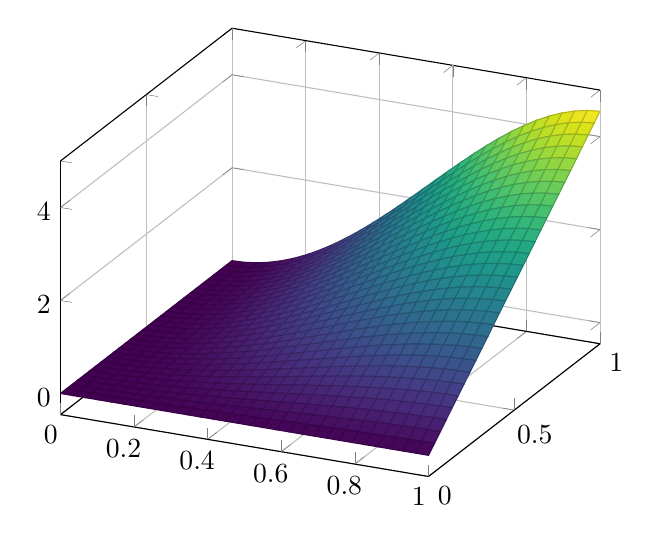
\begin{tikzpicture}
\begin{axis}[grid=major,colormap/viridis,]

\addplot3 [surf,samples=30,domain=0:1,] {5*x*sin(2*deg(x)) * y};

\end{axis}
\end{tikzpicture}}
\end{wrapfigure}

\textit{Visualize 3D surfaces, which are--unlike with meshes--filled. Easiest to create with }\texttt{<expression>}\textit{ but can also create with }\texttt{table}\textit{ or }\texttt{coordinates}\textit{. Choosing from various \say{shaders} affords control over color gradients on each patch. }\texttt{Colormaps}\textit{ are inherited from the }\texttt{axis}\textit{, but can be overridden. For lower-level control of color interpolations, set }\href{\docurl\#pgfp./pgfplots/mesh/color:input}{\opt{mesh/color input}}\textit{. This works with }\href{\docurl\#pgfp./pgfplots/z:buffer}{\opt{mesh}}\textit{, }\href{\docurl\#pgfp./pgfplots/patch}{\opt{patch}}\textit{ or }\href{\docurl\#pgfp./pgfplots/surf}{\opt{surf}}\textit{.}





%%%%%%%%%%%%%%%%%%%%%%%%%%%%%%%%%%%%%%%%%%%%%%%%%%%
\subsection*{\href{\docurl\#pgfp./pgfplots/patch}{Patch}}

\begin{comment}

\begin{wrapfigure}[5]{r}{2.2cm}
\vspace{-8mm}
\resizebox{2cm}{!}{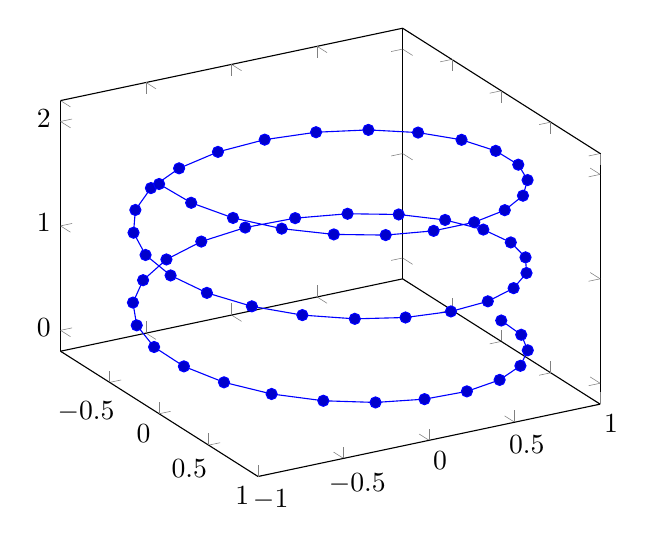
\begin{tikzpicture}
\begin{axis}[view={60}{30}]

\addplot3+ [domain=0:5*pi,samples=60,samples y=0,] ({sin(deg(x))},{cos(deg(x))},{2*x/(5*pi)});

\end{axis}
\end{tikzpicture}}
\end{wrapfigure}

\blindtext
\end{comment}


%%%%%%%%%%%%%%%%%%%%%%%%%%%%%%%%%%%%%%%%%%%%%%%%%%%%
\subsection*{Regression}

